%!TEX root = ./../../../thesis-format/main.tex
	
\IN{slowly synchronizing automaton}
\IN{slowly synchronizing family of automata}
In~\cite{DBLP:conf/mfcs/AnanichevGV10,KisielewiczS15} an automaton
was called \emph{slowly synchronizing}
if ``[...][its] reset length [is] close to 
the \v{C}ern\'y bound [...]''~\cite{DBLP:conf/mfcs/AnanichevGV10}. 
We adhere to this intuitive ``non-quantitative'' definition.
%To exclude 
%certain modifications (similar as in \cref{syncmax:slowly:ex}), 
In~\cite{AnaVolGus2013}
the authors focused on slowly synchronizing $n$-state automaton with reset
lengths between $(n-2)^2 + 2$ and $(n-1)^2$.
In~\cite{Martugin08,DBLP:journals/jalc/Volkov19a}
slowly synchronizing automata whose reset lengths
do not fall within these bounds have been given.
%Here, we adopt the first definition, which is, strictly
%speaking, more an intuitive statement as ``closeness'' is not precisely defined.
%The examples we present
%also obey the more precise definition.
As we are dealing mainly with families of automata
and to formulate two conjectures, %in \cref{sync_max:sec:slowly_sync_discussion}, 
we introduce \emph{slowly synchronizing families of automata}
as infinite families of distinct automata $\semiautomat{A_n}{Q_n}{\Sigma}{\delta_n}$ 	
such that $\rt{\mathcal A_n} \ge C\cdot |Q_n|^2$
for some $C > 0$ and all $n \ge 1$ (most of the time we have $|Q_n| = n$).\footnote{We denote
the alternating group also with $\mathcal A_n$, see \pageref{def:A_n}.
But there should no confusion arise since the context makes it clear whether
we denote an automaton family or the alternating group by~$\mathcal A_n$.} 

%infinitely many $n \ge 1$. 
For example, the \Cerny family~$\mathcal C_n$ from 
\cref{intro:sec:cerny} (\cref{intro:fig:cerny})
is slowly synchronizing.
%Without having a precise definition, 
For any reasonable interpretation of slowly synchronizing automata,
we would expect every family of slowly synchronizing automata
to give a slowly synchronizing family of automata.

In \cref{sync_max:sec:cerny_bound}, 
we discuss automata whose reset lengths reach 
the \v{C}ern\'y bound. In \cref{sync_max:sec:slowly_sync}
we investigate certain known families of slowly synchronizing automata
and observe that for them
%we investigate slowly synchronizing automata and observe that for
%the ones we investigate, 
minimal automata for their sets of synchronizing words are exponentially larger (we also confirm
sync-maximality for the automata~$\mathcal K_n$ for which this was previously only conjectured).
\Cref{sync_max:sec:slowly_sync_discussion} concludes by discussing and formulating conjectures based
on our observations.
%based
%on notions that exclude artificial examples that arise out of adding letters.

\section{Automata Reaching the \Cerny Bound}
\label{sync_max:sec:cerny_bound}

Besides the \Cerny family from \cref{intro:fig:cerny},
for $n \ge 3$,
only the eight exceptional synchronizing $n$-state automata from \cref{sync_max:fig:exceptional_automata}
are known to have reset length $(n-1)^2$
and the property of becoming non-synchronizing after the removal of any letter~\cite{DonZB21,DBLP:conf/lata/Volkov08}.
These exceptional automata are given in \cref{sync_max:fig:exceptional_automata}.
The automaton $\mathbf{K}$ was
discovered by Kari~\cite{JKari01}, the automaton~$\mathbf{I}$ by Roman~\cite{DBLP:journals/jalc/Roman08},
and the remaining six automata by Trahtman via a computer search~\cite{DBLP:conf/mfcs/Trahtman06}.

By extensive compute analysis, Don et al~\cite{DonZB21} 
found $19$ additional automata with at least three and at most six states reaching the \v{C}ern\'y bounds,
but they do not have the property of becoming
non-synchronizing after removal of any letter. In this sense, with these $8$ exceptional automata
and the~$4$ automata from the \Cerny family we have $12$ automata
with at least two and at most six states that reach the \Cerny bound
and are minimal w.r.t.~the alphabet.

Here, we investigate the eight automata from \cref{sync_max:fig:exceptional_automata} w.r.t.~sync-maximality.

\begin{figure}
	\centering
	\begin{tabular}{ccc}
		\begin{tikzpicture}
			\node[state] (0) {$0$};
			\node[state, above left  = of 0] (1) {$1$};
			\node[state, above right = of 0] (2) {$2$};
			
			\path[->] (1) edge [bend left,above] node {$a$} (2)
			(2) edge [bend left,right] node {$a$} (0)
			(0) edge [bend left,left] node {$a,c$} (1);
			\path[->]  (1) edge [bend left,above,pos=.7] node {$c$} (0)
			(2) edge [above] node {$c$} (1);
		\end{tikzpicture}   & &
		
		\begin{tikzpicture}
			\node[state] (0) {$0$};
			\node[state, above left  = of 0] (1) {$1$};
			\node[state, above right = of 0] (2) {$2$};
			
			\path[->] (1) edge [bend left,above] node {$a,b$} (2)
			(2) edge [above] node {$a,b$} (1);
			\path[->] (0) edge [above,pos=.4] node {$c$} (2)
			(2) edge [bend left,below] node {$c$} (0);
			\path[->] (0) edge [above,pos=.4] node {$a$} (1)
			(0) edge [loop left] node {$b$} (0)
			(1) edge [loop left] node {$c$} (1);			 
		\end{tikzpicture}
		
		\\ [2pt]
		The automaton \textbf{D} & & The automaton \textbf{E} \\ [2pt]
		
		\begin{tikzpicture}
			\node[state] (0) {$0$};
			\node[state, right = of 0] (1) {$1$};
			\node[state, right = of 1] (2) {$2$};
			
			\path[->] (0) edge [loop above] node {$c$} (0)
			          (1) edge [loop above] node {$a$} (1)
			          (1) edge [bend left,above]  node {$c$} (2)
			          (2) edge [loop above] node {$a,b$} (2);
			          
			\path[->] (2) edge [bend left,below] node {$c$} (1)
			 (1) edge [bend left,below] node {$b$} (0)
			 (0) edge [bend left,above] node {$a,b$} (1);
 		\end{tikzpicture} & &
		
		\begin{tikzpicture}
			\node[state] (0) {$0$};
			\node[state, right = of 0] (1) {$1$};
			\node[state, right = of 1] (2) {$2$};
			\node[state, above = of 1] (3) {$3$};
			
			\path[->] (0) edge [loop above] node {$a$} (0)
			 (0) edge [above] node {$b$} (3)
			 (1) edge [above] node {$b$} (0)
			 (3) edge [right] node {$b$} (1)
			 (1) edge [bend left,above] node {$a$} (2)
			 (2) edge [bend left,below] node {$a$} (1)
			 (2) edge [loop above] node {$b$} (2)
			 (3) edge [above] node {$a$} (2);
			
		\end{tikzpicture} \\ [2pt]
		
		The automaton \textbf{F} & & The automaton \textbf{G} \\ [2pt]
		
		\begin{tikzpicture}
			\node[state] (2) {$2$};
			\node[state, above left  = of 2] (0) {$0$};
			\node[state, below left  = of 2] (1) {$1$};
			\node[state, right = of 2]       (3) {$3$};
			
			\path[->] (0) edge [left] node {$a$} (1)
			(1) edge [bend left,below] node {$a$} (2)
			(2) edge [bend left,below] node {$a$} (1)
			(3) edge [loop above] node {$a,b$} (3);
			
			\path[->] (0) edge [loop left] node {$c$} (0)
			  (1) edge [loop left] node {$b,c$} (1);
			  
			\path[->] (2) edge [bend left,above] node {$c$} (3)
			 (3) edge [bend left,below] node {$c$} (2)
			 (2) edge [bend left,above] node {$b$} (0)
			 (0) edge [bend left,above] node {$b$} (2);
		\end{tikzpicture} & &
		
		\begin{tikzpicture}
			\node[state] (0) {$0$};
			\node[state, right = of 0] (1) {$1$};
			\node[state, right = of 1] (2) {$2$};
			\node[state, above = of 0,yshift=1.4cm] (3) {$3$};
			
			%\path[<->] (0) edge [above] node {$c$} (3); % zwei pfeile
			\path[->] (0) edge [bend left,left] node {$c$} (3)
			 (3) edge [left] node {$c$} (0);
			
			\path[->] (3) edge [left,pos=0.7] node {$a,b$} (1);
			\path[->] (1) edge [bend right, left] node {$b$}   (3);
			\path[->] (0) edge [loop left] node {$b$} (0)
			          (0) edge [above] node {$a$} (1);
			\path[->] (1) edge [bend left, above] node {$a,c$} (2)
			 (2) edge [bend left, below] node {$c$} (1)
			 (2) edge [loop above] node {$b$} (2)
			 (2) edge [bend right,above] node {$a$} (3);
			 			
		\end{tikzpicture} \\ [2pt]
		The automaton \textbf{H} & & The automaton \textbf{I} \\ [2pt]
		
		\begin{tikzpicture}
			\node[state] (0) {$0$};
			\node[state, above right = of 0] (1) {$1$};
			\node[state, below right = of 0] (2) {$2$};
			\node[state, right = of 1] (4) {$4$};
			\node[state, right = of 2] (3) {$3$};
			
			\path[->] (0) edge [loop above] node {$c$} (0)
			(1) edge [bend left,above] node {$c$} (4)
			(4) edge [bend left,below] node {$c$} (1)
			(2) edge [bend left,above] node {$c$} (3)
			(3) edge [bend left,below] node {$c$} (2);
			
			\path[->] (0) edge [above] node {$b$} (2)
			(2) edge [bend left,below]  node {$b$} (0)
			(3) edge [loop right] node {$a,b$} (3)
			(4) edge [loop right] node {$a,b$} (4)
			(1) edge [loop left] node {$b$} (1);
			
			\path[->] (0) edge [above,below] node {$a$} (1)
			(1) edge [bend left,right] node {$a$} (2)
			(2) edge [left] node {$a$} (1);			 
		\end{tikzpicture} & &
		
		\begin{tikzpicture}
		%	\tikzstyle{state}=[minimum size=25pt,inner sep=1pt];
			\node[state] (0) {$0$};
			\node[state, right = of 0] (1) {$1$};
			\node[state, right = of 1] (2) {$2$};
			\node[state, below = of 2, yshift=-1.3cm] (3) {$3$};
			\node[state, left = of 3]  (4) {$4$};
			\node[state, left = of 4]  (5) {$5$};			
			
			\path[->] (0) edge [above] node {$a$} (1) 
			 (1) edge [above] node {$a$} (2) 
			 (2) edge [bend right,above] node {$a$} (0);
			 
			\path[->] (5) edge [above] node {$a$} (4)
			 (4) edge [above] node {$a$} (3)
			 (3) edge [bend left, below] node {$a$} (5);
			 
			\path[->] (0) edge [loop above] node {$b$} (0)
			 (1) edge [loop below] node {$b$} (1)
			 (2) edge [bend left, right]  node {$b$} (3)
			 (3) edge [bend left, right]  node {$b$} (2)
			 (4) edge [left] node {$b$} (2)
			 (5) edge [loop above] node {$b$} (5);
			
		\end{tikzpicture} \\ [2pt]
		
		Roman's automaton \textbf{J} & & Kari's automaton \textbf{K}.
		
	\end{tabular}
	\caption[Eight exceptional automata attaining the \v{C}ern\'y bound]{The eight exceptional automata whose reset lengths equal the \v{C}ern\'y bound $(n-1)^2$. 
	The naming is taken from~\cite{HeCLS21} (a mistake for \textbf{J} in~\cite{HeCLS21} has been fixed here, the correct automaton is written in~\cite{DBLP:conf/lata/Volkov08}).} \label{def:exceptional_aut}
	\label{sync_max:fig:exceptional_automata}
\end{figure}

\begin{figure}
\centering 
\scalebox{0.975}{
\begin{tikzpicture}[shorten >=1pt,->,node distance=1.25cm]
	\tikzstyle{state-subset}=[]
	
	\node[state-subset, initial, initial where=right] (0123) {$\{0,1,2,3\}$};
	\node[state-subset, below = of 0123, yshift=0.5cm] (123) {$\{1,2,3\}$};
	\node[state-subset, below = of 123]  (012) {$\{0,1,2\}$};
	\node[state-subset, right = of 012]  (023) {$\{0,2,3\}$};
	\node[state-subset, above = of 023]  (013) {$\{0,1,3\}$};
	\node[state-subset, right = of 023]  (13)  {$\{1,3\}$};
	\node[state-subset, above = of 13]   (12)  {$\{1,2\}$}; 
	\node[state-subset, right = of 12]   (23)  {$\{2,3\}$};
	\node[state-subset, right = of 13]   (02)  {$\{0,2\}$};
	\node[state-subset, right = of 23]   (01)  {$\{0,1\}$};
 	\node[state-subset, below = of 01]   (03)  {$\{0,3\}$};
 	\node[state, fill=white,minimum size=17pt,inner sep=1pt, below = of 03, accepting]   (1)   {$*$}; % genügt, sagen einermenge kollapsed, vielleicht mit * andeuteen
 	
 	\path[->] (0123) edge [right] node {$a$} (123)
 	          (0123) edge [loop left,looseness=2.5] node {$b,c$} (0123);
 	          
 	\path[->] (123) edge [loop left,looseness=2] node {$a,b$} (123)
 	          (013) edge [above] node {$a$} (12)
 	          (023) edge [above] node {$a$} (13);
 	\path[->] (012) edge [bend left,left] node {$a$} (123);
 	
 	\path[->] (12) edge [bend left, above] node {$a$} (23)
 	          (23) edge [bend left, above] node {$a$} (13)
 	          (13) edge [left] node {$a$} (12);
 	          
   \path[->] (01) edge [bend right,above,out=300,in=230] node {$a$} (12)
             (03) edge [right] node {$a$} (1);
   \path[<->] (02) edge [below] node {$c$} (13);
   \path[->]  (02) edge [bend left, below] node {$a$} (13);
             
    \path[<->] (123) edge [right] node {$c$} (012)
               (023) edge [above] node {$b$} (012)
               (013) edge [left] node {$c$} (023);
     
    \path[->] (013) edge [loop left,looseness=2] node {$b$} (013)
              (13)  edge [loop below] node {$b$} (13)
              (12)  edge [loop above] node {$c$} (12);
              
    \path[<->] (23) edge [below] node {$b$} (12)
               (02) edge [loop below] node {$b$} (02)    
               (01) edge [right] node {$b$} (03)
               (01) edge [above] node {$c$} (23);  
    \path[->] (03) edge [loop right,looseness=3] node {$c$} (03);     
    \path[->] (1) edge [loop left] node {$a,b,c$} (1);           
\end{tikzpicture}
}
\caption[Minimal automaton for $\Syn(\mathbf{I})$]{A minimal automaton for the set of synchronizing word of the automaton $\textbf{I}$ from Figure~\ref{sync_max:fig:exceptional_automata}. See the proof of Theorem~\ref{sync_max:thm:extremal_automata} for details.}
\label{sync_max:fig:I} % final und start adden
\end{figure}

\begin{theorem}
\label{sync_max:thm:extremal_automata}
Consider the exceptional automata for the \v{C}ern\'y bound from \FIG~\ref{sync_max:fig:I}.
	The automata \textbf{D}, \textbf{E}, \textbf{I} and \textbf{F} are sync-maximal.
	\textbf{G}, \textbf{H}, \textbf{J} and \textbf{K} are not sync-maximal.
\end{theorem}
\begin{proof} We handle each automaton individually.
		
	\begin{enumerate}
		\item[\textbf{D}, \textbf{E}, \textbf{F}:] In \textbf{D} the letter $a$ generates a primitive permutation group;
		in \textbf{E} and \textbf{F} the letters~$b$ and~$c$ generate the full symmetric group on $\{0,1,2\}$ in the transformation semigroup,
		which is primitive.		
		So, in all cases, sync-maximality follows from \cref{sync_max:thm:prim}.
				
		For \textbf{E}, we also obtain sync-maximality directly by observing that
		$a$ has image $\{1,2\}$, $ac$ has image $\{0,1\}$, $acb$ has image $\{0,2\}$, $acba$ has image $\{1\}$, 
		and since we have the following distinguishing words for all pairs:
		\begin{center}
		\begin{tabular}{l|c|l|c}
			Pair of Subsets & Dist. Word & Pair of Subsets & Dist. Word \\ \hline 
			$\{0,2\}$, $\{1,2\}$    & $a$ & $\{0,1\}$, $\{1,2\}$    & $ba$   \\
			$\{0,2\}$, $\{0,1\}$    & $a$ &	$\{0,1,2\}$, $\{0,1\}$  & $ba$   \\
			$\{0,2\}$, $\{0,1,2\}$  & $a$ &	$\{0,1,2\}$, $\{1,2\}$  & $cba$ \\
		\end{tabular}
	    \end{center}
		For \textbf{E}, we have that $a$, $ab$, $abc, abca$ map $\{0,1,2\}$ to $\{1,2\}, \{0,2\}$, $\{0,1\}$ and $\{1\}$ respectively.
		Furthermore, $a$ distinguishes $\{0,1\}$ form every other $2$-set,
		and $ca$ distinguishes $\{1,2\}$ from $\{0,2\}$.
		
		\item[\textbf{G}:] The following diagram shows the reachable $3$-sets:
		\begin{center}	
			\begin{tikzpicture}[>=stealth, every node/.style={font=\small}]			
				\matrix (m) [matrix of math nodes, column sep=2em] {
					\{0,1,2,3\} & \{0,1,2\} & \{0,2,3\} & \{1,2,3\} \\
				};
				
				\path[->] (m-1-1) edge[above] node {$a$} (m-1-2);
				\path[->] (m-1-2) edge[loop above, in=60, out=120, looseness=3] node {$a$} (m-1-2);
				
				\path[->] (m-1-2) edge[bend left=10,above] node {$b$} (m-1-3);
				\path[->] (m-1-3) edge[bend left=10,below] node {$a$} (m-1-2);
				
				\path[->] (m-1-3) edge[above] node {$b$} (m-1-4);
			\end{tikzpicture}
		\end{center}
		Since $\{0,1,3\}$ is not reachable, the automaton is not sync-maximal by \cref{sync_maximal:thm:structure}.
				
		\item[\textbf{H}:] The following diagram shows all reachable $3$-sets:
		\begin{center}	
		\begin{tikzpicture}[>=stealth, every node/.style={font=\small}]
			
			\matrix (m) [matrix of math nodes, column sep=2em] {
				\{0,1,2,3\} & \{1,2,3\} & \{0,1,3\} & \{0,1,2\} \\
			};
			
			\path[->] (m-1-1) edge[above] node {$a$} (m-1-2);
			\path[->] (m-1-2) edge[loop above, in=60, out=120, looseness=3] node {$a,c$} (m-1-2);
			\path[->] (m-1-2) edge[bend left=10, above] node {$b$}   (m-1-3);
			\path[->] (m-1-3) edge[bend left=10, below] node {$a,b$} (m-1-2);
			\path[<->] (m-1-3) edge[above] node {$c$} (m-1-4);
			\path[->] (m-1-4) edge[loop above, in=60, out=120, looseness=3] node {$b$} (m-1-4);
		\end{tikzpicture}
		\end{center}
		We see that not all $3$-sets are reachable. So, the strongly connected automaton~$\text{H}$ 
		is not sync-maximal  by \cref{sync_maximal:thm:structure}.
		
		\item[\textbf{I}:] 
		The word $b$ induces a transposition and the word $cb$
		induces the cycle $(0 ~ 1 ~ 2 ~ 3)$.
		Thus by \cref{prelim:thm:cycles_gen_Sn} the 
		transformation semigroup contains
		the full symmetric group.
		Since the full symmetric group is primitive,
		from \cref{sync_max:thm:prim} 
		we find that the automaton is sync-maximal.
				
		For an alternative proof, consider the power automaton
		 with the singleton sets merged into a single state and the empty set omitted
		 shown in \cref{sync_max:fig:I}.
		 We see that $\textbf{I}$ is completely reachable.
		 Now, the words $u_1 = aacba$, $u_2 = au_1$, $u_3 = bu_2$, and $u_4 = cu_3$ 
		 map $\{0,1,3\}$, $\{0,2,3\}$, $\{0,1,2\}$, and $\{1,2,3\}$, respectively,
		 to a singleton while mapping the state not in the respective
		 set to another distinct state.
		 So, by \crefitem{sync_max:thm:char_distinguishable}{dist:item:single_point},
		 the automaton \textbf{I} is completely distinguishable.
		 By \cref{sync_maximal:thm:structure}, $\textbf{I}$ is sync-maximal.
		 			
		\item[\textbf{J}:] 
		We have the following transitions from the whole state set 
		(omitting transitions into sets with less than four elements):		
		\begin{center}	
			\begin{tikzpicture}[>=stealth, every node/.style={font=\small}]
				
				\matrix (m) [matrix of math nodes, column sep=2em] {
					\{0,1,2,3,4\} & \{1,2,3,4\} & \{0,1,3,4\} & \{0,1,2,4\} \\
				};
				
				\path[->] (m-1-1) edge[above] node {$a$} (m-1-2);
				\path[->] (m-1-2) edge[loop above, in=60, out=120, looseness=3] node {$a$} (m-1-2);
				\path[<->] (m-1-2) edge[above] node {$b$} (m-1-3);
				\path[<->] (m-1-3) edge[above] node {$c$} (m-1-4);
				\path[->] (m-1-4) edge[loop above, in=60, out=120, looseness=3] node {$b$} (m-1-4);
			\end{tikzpicture}
		\end{center}
		Since $\{0,1,2,3\}$ is not reachable,~$\textbf{J}$ is not sync-maximal by \cref{sync_maximal:thm:structure}.
	
		\item[\textbf{K}:] All the reachable $5$-sets are 
		$\{0,1,2,3,5\}$,$\{0,1,2,4,5\}$, and $\{0,1,2,3,4\}$.
		Thus, not all $5$-sets are reachalbe.
		Since, by \cref{sync_maximal:thm:structure}, for strongly connected automata,
		complete reachability is a necessary condition for sync-maximality, 
		$\textbf{K}$ is not sync-maximal.~\qedhere 	
	\end{enumerate}
\end{proof}

\begin{remark}
	In \textbf{J}, 
	the letters~$b$ and~$c$ restricted to $\{0,2,3\}$
	generate the full symmetric group on $\{0,2,3\}$.
	Since~$a$ maps $\{0,1,2\}$ to $\{1,2\}$,
	we can conclude that the subsets of the form $A \cup \{1,4\}$
	with $A \subseteq \{0,2,3\}$
	form a family of reachable and pairwise distinguishable subsets.
		
	In \textbf{K}, the letters $a$ and $bb$
	induce a subautomaton on $\{3,4,5\}$
	that is isomorphic to the \v{C}ern\'y automaton on three states
	and since $a$ and $b$ permute $\{0,1,2\}$
	the sets of the form $A \cup \{0,1,2\}$
	with $A \subseteq \{3,4,5\}$
	form a  family of reachable and pairwise distinguishable subsets.
\end{remark}

\section{Families of Slowly Synchronizing Automata}
\label{sync_max:sec:slowly_sync}

Here, we present a couple of slowly synchronizing families of automata from the literature and investigate 
the size of their minimal automata for the set of synchronizing words. 

\Cref{tab:slowly_sync_families} shows slowly synchronizing automata
which we show to be sync-maximal in \cref{sync_max:thm:families}.
We only give the state diagrams, the formal definitions should be clear from these diagrams.
For example, the automata family~$\mathcal  K_n = ([n], \Sigma, \delta_n)$
($n > 5$ odd) is defined\footnote{The numbering of the states w.r.t.~the letter~$a$	has been changed compared to ~\cite{DBLP:journals/ijfcs/Maslennikova19}.}
by
\begin{align*} 
	%\delta(i, b) & = i + 1 \mbox{ for } i \in \{0,\ldots, n-2\}, \mbox{ and } \delta(n-1, b) = 0, \\
	\delta_n(i, b) & = (i + 1) \bmod{n} \mbox{ for } i \in \{0,\ldots,n-1\}, \\
	\delta_n(i, a) & = (i + 1) \bmod{n} \mbox{ for } i \in \{1, \ldots,n-3,n-1\}, \\
	\delta_n(n-2,a) & = 1 \text{ and } 	\delta_n(0,a) = 3.
\end{align*}
For the families from \cref{tab:slowly_sync_families},  except for~$\mathcal K_n$ (for which
this was an open problem), sync-maximality has been shown
in~\cite{DBLP:journals/ijfcs/Maslennikova19} by rather involved arguments.\footnote{For $\mathcal V_n$
	sync-maximality follows readily by considering $a^{n-1}$ and $b$ as letters, as the resulting
	automaton is isomorphic to the \v{C}ern\'y automaton.}
By our general results this result follows readily. 




% https://tex.stackexchange.com/questions/7208/how-to-vertically-center-the-text-of-the-cells
% https://stackoverflow.com/questions/25163873/horizontal-and-vertical-alignment-in-tabular-cell
\begin{table}[th]
    \centering
    \caption[Slowly synchronizing and sync-maximal $n$-state automata]{Slowly synchronizing and sync-maximal automata. 
    	Names from the literature and reset lengths are indicated. 
    	The marked state is used to deduce sync-maximality via \THM~\ref{sync_max:thm:circular_sync_max} in the proof of \THM~\ref{sync_max:thm:families}.
    	%Additionally, every primitive group
    	%together with a non-permutation of rank $n - 1$ yields such extremal automata for the set of synchronizing words~\cite{zweiarbeiten.}.
    } 
 \begin{tabular}{c|c|c|c}%p{2.2cm}} 
 \hline 
  Name & Automata & Reset Length & Referenz \\ \hline
  $\mathcal C_n$ & 
  \begin{tabular}{l}
   \rule[-0.02cm]{0pt}{2.15cm}
 \scalebox{.8}{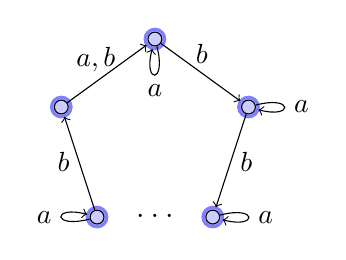
\begin{tikzpicture}[shorten >=1pt,->,node distance=4cm]
  %\tikzstyle{vertex}=[circle,color=red!60,fill=black!10,minimum size=25pt,inner sep=1pt,very thick]
  \tikzstyle{vertex}=[circle,draw,minimum size=5pt,inner sep=1pt]
 
  \foreach \name/\angle/\text in {P-n-2/234/n-2, P-n-1/162/n-1, 
                                  P-0/90/0, P-1/18/1, P-2/-54/2}
{
	\ifthenelse{\equal{\angle}{162}}
	{
		\node[circle,draw,minimum size=7pt,inner sep=1pt,draw=blue!50,very thick,fill=blue!20] (\name) at (\angle:1.25cm) {};
	}
	{
		\node[vertex] (\name) at (\angle:1.25cm) {};
	}
}

  % \node at (0, -1.5) {$\ldots$};

   \path[->] (P-n-2) edge [left] node {$b$} (P-n-1);
   \path[->] (P-n-1) edge [above,pos=0.35] node {$a,b$} (P-0);
   \path[->] (P-0) edge [above] node {$b$} (P-1);
   \path[->] (P-1) edge [right] node {$b$} (P-2);
   
   \path[->] (P-n-2) edge [loop left] node {$a$} (P-n-2);
   \path[->] (P-0) edge [loop below] node {$a$} (P-0);
   \path[->] (P-1) edge [loop right] node {$a$} (P-1);
   \path[->] (P-2) edge [loop right] node {$a$} (P-2);
   
  \node at (0, -1) {\large $\ldots$};
\end{tikzpicture}}%
\end{tabular} & $(n-1)^2$ & %Transforms to $\mathcal W_n$ with $b$ and $c = ab$,
\cite{AnaVolGus2013,Cer64,DBLP:journals/ijfcs/Maslennikova19} \\  \hline
\begin{tabular}{l} 
$\mathcal V_n = \mathcal W_n$ 
\end{tabular}
& 
\begin{tabular}{l} 
 \rule[-0.02cm]{0pt}{2.15cm}
 \scalebox{.8}{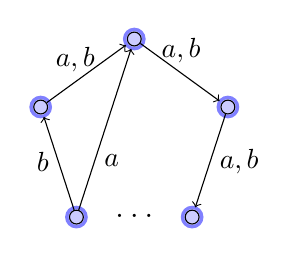
\begin{tikzpicture}[shorten >=1pt,->,node distance=5cm]
  \tikzstyle{vertex}=[circle,draw,minimum size=5pt,inner sep=1pt]
 
  \foreach \name/\angle/\text in {P-n-2/234/n-2, P-n-1/162/n-1, 
                                  P-0/90/0, P-1/18/1, P-2/-54/2}
{
	\ifthenelse{\equal{\angle}{234}}
	{
		\node[circle,draw,minimum size=7pt,inner sep=1pt,draw=blue!50,very thick,fill=blue!20] (\name) at (\angle:1.25cm) {};
	}
	{
		\node[vertex] (\name) at (\angle:1.25cm) {};
	}
}
   
  % \node at (0, -1.5) {$\ldots$};

  \path[->] (P-n-2) edge [left] node {$b$} (P-n-1);
  \path[->] (P-n-1) edge [above,pos=0.35] node {$a,b$} (P-0);
  \path[->] (P-0) edge [above] node {$a,b$} (P-1);
  \path[->] (P-1) edge [right] node {$a,b$} (P-2);
   
  \path[->] (P-n-2) edge [right,pos=0.3] node {$a$} (P-0);
   
  \node at (0, -1) {\large $\ldots$};
\end{tikzpicture}} 
\end{tabular}
& 
\begin{tabular}{l} $n^2 - 3n + 3$ 
\end{tabular}
& \cite{AnaVolGus2013,DBLP:journals/ijfcs/Maslennikova19}
\\ \hline 
  \begin{tabular}{l}
  $\mathcal L_n = \mathcal D_n'$
  \end{tabular} 
 &
  \begin{tabular}{l} 
   \rule[-0.02cm]{0pt}{2.15cm}
       \scalebox{.8}{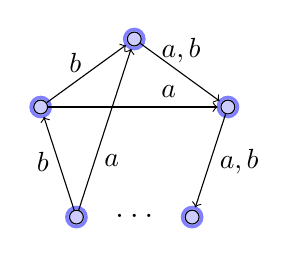
\begin{tikzpicture}[shorten >=1pt,->,node distance=4cm]
  \tikzstyle{vertex}=[circle,draw,minimum size=5pt,inner sep=1pt]
 
  \foreach \name/\angle/\text in {P-n-2/234/n-2, P-n-1/162/n-1, 
                                  P-0/90/0, P-1/18/1, P-2/-54/2}
{
	\ifthenelse{\equal{\angle}{162}}
	{
		\node[circle,draw,minimum size=7pt,inner sep=1pt,draw=blue!50,very thick,fill=blue!20] (\name) at (\angle:1.25cm) {};
	}
	{
		\node[vertex] (\name) at (\angle:1.25cm) {};
	}
}
   
   %\node at (0, -1.5) {$\ldots$};

   \path[->] (P-n-2) edge [left] node {$b$} (P-n-1);
   \path[->] (P-n-1) edge [above,pos=0.35] node {$b$} (P-0);
   \path[->] (P-0) edge [above] node {$a,b$} (P-1);
   \path[->] (P-1) edge [right] node {$a,b$} (P-2);
   
   \path[->] (P-n-2) edge [right,pos=0.3] node {$a$} (P-0);
   \path[->] (P-n-1) edge [above,pos=0.7] node {$a$} (P-1);
   
  \node at (0, -1) {\large $\ldots$};
\end{tikzpicture}}
  \end{tabular}
    & $n^2 - 3n + 4$ & \cite{AnaVolGus2013,DBLP:journals/ijfcs/Maslennikova19}   \\ \hline
\begin{tabular}{l}
$\mathcal F_n$ \\ 
$n > 3$ odd  
\end{tabular} &

\begin{tabular}{l}
 \rule[-0.02cm]{0pt}{2.15cm}
 \scalebox{.8}{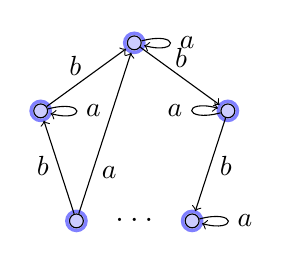
\begin{tikzpicture}[shorten >=1pt,->,node distance=5cm]
  %\tikzstyle{vertex}=[circle,color=red!60,fill=black!10,minimum size=25pt,inner sep=1pt,very thick]
  \tikzstyle{vertex}=[circle,draw,minimum size=5pt,inner sep=1pt]
 
  \foreach \name/\angle/\text in {P-n-2/234/n-2, P-n-1/162/n-1, 
                                  P-0/90/0, P-1/18/1, P-2/-54/2}
{
	\ifthenelse{\equal{\angle}{234}}
	{
		\node[circle,draw,minimum size=7pt,inner sep=1pt,draw=blue!50,very thick,fill=blue!20] (\name) at (\angle:1.25cm) {};
	}
	{
		\node[vertex] (\name) at (\angle:1.25cm) {};
	}
}

   \path[->] (P-n-2) edge [left] node {$b$} (P-n-1);
   \path[->] (P-n-1) edge [above,pos=0.35] node {$b$} (P-0);
   \path[->] (P-0) edge [above] node {$b$} (P-1);
   \path[->] (P-1) edge [right] node {$b$} (P-2);
   
   \path[->] (P-n-2) edge [right,pos=0.25] node {$a$} (P-0);
   \path[->] (P-n-1) edge [loop right] node {$a$} (P-n-1);
   \path[->] (P-0) edge [loop right] node {$a$} (P-0);
   \path[->] (P-1) edge [loop left] node {$a$} (P-1);
   \path[->] (P-2) edge [loop right] node {$a$} (P-2);
   \node at (0, -1) {\large $\ldots$};
\end{tikzpicture}}
\end{tabular}
& $n^2 - 3n + 3$ & \cite{AnaVolGus2013,DBLP:journals/ijfcs/Maslennikova19} \\ \hline
\begin{tabular}{l}
$\mathcal K_n = \mathcal G_n$ \\  $n > 5$ odd
\end{tabular}
 & 
\begin{tabular}{l}
 \rule[-0.02cm]{0pt}{2.15cm}
\scalebox{.8}{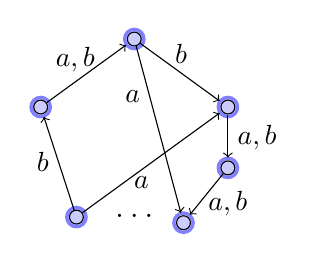
\begin{tikzpicture}[shorten >=1pt,->,node distance=5cm]
  \tikzstyle{vertex}=[circle,draw,minimum size=5pt,inner sep=1pt]
 
  \foreach \name/\angle/\text in {P-n-2/234/n-2, P-n-1/162/n-1, 
                                  P-0/90/0, P-1/18/1, P-2/-18/2, P-3/-60/3}
{
	\ifthenelse{\equal{\angle}{90}}
	{
		\node[circle,draw,minimum size=7pt,inner sep=1pt,draw=blue!50,very thick,fill=blue!20] (\name) at (\angle:1.25cm) {};
	}
	{
		\node[vertex] (\name) at (\angle:1.25cm) {};
	}
}
   
   \node at (0, -1) {\large $\ldots$};

   \path[->] (P-n-2) edge [left] node {$b$} (P-n-1);
   \path[->] (P-n-1) edge [above,pos=0.35] node {$a,b$} (P-0);
   \path[->] (P-0) edge [above] node {$b$} (P-1);
   \path[->] (P-1) edge [right] node {$a,b$} (P-2);
   \path[->] (P-2) edge [right,pos=0.7] node {$a,b$} (P-3);
   
   \path[->] (P-n-2) edge [right,pos=0.3] node {$a$} (P-1);
   \path[->] (P-0) edge [left,pos=0.3] node {$a$} (P-3);
\end{tikzpicture}}
\end{tabular}
& $n^2 - 4n + 7$ & \begin{tabular}{l} Thm.~\ref{sync_max:thm:families} \& \\ \cite{AnaVolGus2013,DBLP:journals/ijfcs/Maslennikova19} \end{tabular} \\ \hline
%- & Primitive Group + Rank $n - 1$ Non-Permutation & - & \cite{Hoffmann20}
\end{tabular}
    \label{def:Vn}\label{def:Ln}\label{def:Fn}\label{def:Kn}
    \label{tab:slowly_sync_families}
\end{table}

\todo[inline]{noch farblich makrieren wie in STACS paper} 

% https://tex.stackexchange.com/questions/87975/one-figure-having-two-columns-of-subfigures-the-left-column-has-one-image-and-t
\newsavebox{\measurebox}
\begin{figure}[th]
	\centering
	\sbox{\measurebox}{%
		\begin{minipage}[b]{.45\textwidth}
			\subfloat
			[$\overline{\mathcal{M}}_n$ ($n$ even and $n \ge 8$) from~\cite{Martugin08}
			%with $\rt{\mathcal{M}_n} = \frac{n^2 + 6n - 16}{4}$ ($n$ even).
			with reset length $\frac{n^2 + 6n - 16}{4}$.
			]
			{\label{sync_max:fig:An}
		\scalebox{0.85}{
			\begin{tikzpicture}
			%	\tikzstyle{state}=[circle,draw,minimum size=30pt,inner sep=1pt]
				%\tikzstyle{state}=[blur shadow,fill={rgb:black,0.4;white,10},minimum size=30pt,inner sep=1pt]
				\tikzstyle{state}=[circle,draw,blur shadow,fill={rgb:black,0.4;white,10},minimum size=30pt,inner sep=1pt]				
				
				\node[state, xshift=-2.3cm] (0) {$0$};
				\node[state, right = of 0, xshift=-0.5cm] (1) {$1$};
				\node[state, right = of 1, xshift=-0.5cm] (2) {$2$};
				%\node[right = of 2] (dots) {$\ldots$};
				\node at (1.8,0) (dots) {$\ldots$};
				\node[state, right = of dots,xshift=-1cm] (m-2) {$m-2$}; 
				\node[state, right = of m-2, xshift=-0.4cm]  (m-1) {$m-1$};
				%\node[state, below right = of dots] (m) {$m$};
				%\node[state] at (8,-2) (m) {$m$};
				\node[state, below = of dots,xshift=-0.5cm,yshift=-0.3cm] (m) {$m$};
				\node[state, below right = of m] (2m-2) {$2m-2$};
				\node[state, below = of 2m-2] (2m-3) {$2m-3$};
				\node[state, below left = of 2m-3] (m+3) {$m+3$};
				\node[state, above left = of m+3] (m+2) {$m+2$};
				\node[state, below left = of m] (m+1) {$m+1$};
				\node[state, left = of m+1,xshift=0.5cm] (2m-1) {$2m-1$}; 
				
				\node at (2.35,-7.25) {$\reflectbox{$\ddots$}$};
				
				% blau b, a rot?
				
				\path[->] (0) edge [loop below] node {$a,b$} (0);
				\path[->] (1) edge [above] node {$a$} (0);
				\path[->] (2) edge [above] node {$a$} (1);
				\path[->] (m-1) edge [above] node {$a$} (m-2);
				\path[->] (1) edge [below] node {$b$} (m);
				\path[->] (2) edge [left] node {$b$} (m);
				\path[->] (m-2) edge [left] node {$b$} (m);
				%	\path[->] (m-1) edge [below,bend left] node {$b$} (m);
				\path[->] (m)   edge [below,bend right=40] node {$b$} (m-1);
				\path[->] (m-1) edge [above,pos=0.7,bend left=15] node {$b$} (m);
				
				\path[->] (2m-1) edge [loop above] node {$a$} (2m-1);
				\path[->] (m+1)  edge [above] node {$b$} (2m-1);
				\path[->] (2m-1) edge [below] node {$b$} (m+2);
				\path[->] (m+2)  edge [left] node {$a$} (m+1);
				\path[->] (m+2)  edge [above,bend left] node {$b$} (m+3);
				\path[->] (m+3)  edge [below,bend left] node {$a$} (m+2);
				\path[->] (2m-3) edge [left, bend left] node {$b$} (2m-2);
				\path[->] (2m-2) edge [right, bend left] node {$a$} (2m-3);
				\path[->] (2m-2) edge [above] node {$b$} (m+1);
				\path[->] (m) edge [right] node {$a$} (2m-2);
				\path[->] (m+1) edge [above] node {$a$} (m);
				
				%\node at (1.5,-5.5) {$\overline{\mathcal A}_n$ ($n$ even)};
			\end{tikzpicture}
		}	
				
		}	
	\end{minipage}}
	\usebox{\measurebox}\qquad
	\begin{minipage}[b]{.45\textwidth}
		\centering
		\subfloat
		[$\mathcal M_n$ ($n \ge 3$)
		with reset length $n^2 - 3n + 3$  introduced in~\cite{KisielewiczS15}.]
		{\label{sync_max:fig:Mn}
	\scalebox{.85}{\begin{tikzpicture}[shorten >=1pt,->,node distance=5cm]
			%\tikzstyle{vertex}=[circle,draw,minimum size=25pt,inner sep=1pt]
			\tikzstyle{vertex}=[circle,draw,blur shadow,fill={rgb:black,0.4;white,10},minimum size=25pt,inner sep=1pt]
			
			
			\foreach \name/\angle/\text in {P-n-2/234/n-2, P-n-1/162/n-1, 
				P-0/90/0, P-1/18/1, P-2/-54/2}
			\node[vertex] (\name) at (\angle:1.75cm) {$\text$};
			
			\path[->] (P-0)   edge [below, pos=0.3,bend left=10] node {$c$} (P-n-1)
			(P-n-1) edge [above, bend left=10] node {$c$} (P-0);
			
			\path[->] (P-1) edge [loop right]   node {$b,c$} (P-1);
			\path[->] (P-2) edge [loop right]   node {$b,c$} (P-2);
			\path[->] (P-n-2) edge [loop left] node {$b,c$} (P-n-2);
			\path[->] (P-n-1) edge [loop left] node {$b$} (P-n-1);
			
			\path[->] (P-n-1) edge [below] node {$a$} (P-1);
			
			\path[->] (P-0) edge [right,pos=.5] node {$a,b$} (P-1)
			(P-1) edge [right] node {$a$}   (P-2)
			(P-n-2) edge [left] node {$a$} (P-n-1);
			\node at (0, -1.5) {\large $\ldots$};			
	\end{tikzpicture}} 
}
		\vfill
		\subfloat
		[$\mathcal B_n$ ($n \ge 5$ odd) from~\cite{AnaVolGus2013,AnanichevVZ07}
		 with reset length $n^2 - 3n + 2$.		 
		%The slowly synchronizing automaton $\mathcal B_n$ ($n \ge 5$ odd) from~\cite{AnanichevVZ07,AnaVolGus2013}.
		%with a shortest synchronizing word of length $n^2 - 3n + 2$. 
		%As it has no letter of defect one it is not sync-maximal.
		]
		{\label{sync_max:fig:Bn}
					\scalebox{.85}{\begin{tikzpicture}[shorten >=1pt,->,node distance=5cm]
						%\tikzstyle{vertex}=[circle,draw,minimum size=10pt,inner sep=1pt]
						\tikzstyle{vertex}=[circle,draw,blur shadow,fill={rgb:black,0.4;white,10},minimum size=25pt,inner sep=1pt]
											
						\foreach \name/\angle/\text in {P-n-2/234/n-2, P-n-1/155/n-1, 
							P-0/90/0, P-1/25/1, P-2/-18/2, P-3/-60/3}
						\node[vertex] (\name) at (\angle:1.85cm) {$\text$};
						
						\path[->] (P-n-1) edge [above] node {$a$} (P-1)
						(P-0)   edge [pos=.8,left] node {$a$} (P-2)
						(P-1)   edge [loop right] node {$a$} (P-1)
						(P-2)   edge [loop right] node {$a$} (P-2)
						(P-3)   edge [loop right] node {$a$} (P-3)
						(P-n-2) edge [loop left]  node {$a$} (P-n-2);						
						
						\path[->] (P-n-2) edge [left] node {$b$} (P-n-1)
						(P-n-1) edge [above] node {$b$} (P-0)
						(P-0)   edge [above] node {$b$} (P-1)
						(P-1)   edge [right] node {$b$} (P-2)
						(P-2)   edge [right] node {$b$} (P-3);
						\node at (0, -1.55) {\large $\ldots$};
				\end{tikzpicture}} 
		}
	\end{minipage}
\caption[Non-sync-maximal and slowly synchronizing automata families]{Slowly synchronizing families
	whose automata are not sync-maximal, but minimal automata for their sets of synchronizing
	words are exponentially larger in the number of states.
	 See the main text for details. %$\mathcal B_n$ is not sync-maximal as it has no letter of defect one. 
} \label{def:overlineAn} \label{def:Mn} \label{def:Bn}
\label{fig:slowly}
\end{figure}

\begin{theorem}
\label{sync_max:thm:families}
	The automata from the families listed in Figure~\ref{tab:slowly_sync_families} are sync-maximal.
\end{theorem}
\begin{proof}
	Let $\semiautomat{A}{Q}{\{a,b\}}{\delta}$.
	For $\mathcal A \in \{\mathcal C_n, \mathcal V_n, \mathcal L_n \}$
	there exists a state~$q$ (marked in \cref{tab:slowly_sync_families})
	such that $\applytrans{\delta}{q}{a} = \applytrans{\delta}{q}{ba}$.
	As the letter $b$ cyclically permutes the states and~$a$ has defect one,
	these automata are sync-maximal by \cref{sync_max:thm:circular_sync_max} 
	(for $\mathcal C_n$, this was also established in \cref{sync_max:thm:cerny_sync_maximal} before).	
	For $\mathcal A \in \{\mathcal F_n, \mathcal K_n\}$ there exists a state~$q$
	such that $\applytrans{\delta}{q}{a} = \applytrans{\delta}{q}{b^2a}$.
	As in this case $n$ is odd, $a$ has defect one, and the letter $b$ cyclically permutes the states,
	sync-maximality follows as well from \cref{sync_max:thm:circular_sync_max}.
\end{proof}

\begin{theorem}
\label{syn_max:thm:An}
  The automata $\overline{\mathcal{M}}_n$ ($n$ even and $n \ge 8$) from~\cref{sync_max:fig:An} introduced in~\cite{Martugin08}\footnote{In~\cite{DBLP:journals/jalc/AnanichevV19} the notation
  	$\mathcal M_n$ was used for this family, that we already used
  	for the family from \cref{sync_max:fig:Mn}.
  	In~\cite{Martugin08} 
  	the notation $\mathcal A_n$ has been used, but we prefer to use
  	$\mathcal A_n$ to denote a general family of automata.}  	  
  are not sync-maximal
  but a minimal automaton for $\Syn(\mathcal{M}_n)$ has at least $2^{n/2}$ states.
 % sogar noch mehr bis auf konstante, wenn man oben die nicht am anfang "rausschiebt"
\end{theorem}
\begin{proof}
	Let $\overline{\mathcal{M}}_n = (Q_n,\{a,b\},\delta_n)$
	with $Q_n = [2m]$ where $m \ge 4$.	
	Since $0$ is a trap state, $\overline{\mathcal{M}}_n$ is not sync-maximal by \cref{syncmax:cor:three-states-trap-not-syncmax}.
	Set $P = \{ m, m +1, \ldots, 2m-1 \}$.
	In the following, we write~$\delta$ 
	for~$\delta_n$ for simplicity.
	Then
	\[
	( \fword{\delta}{babab} )_{| P } = (m ~ m + 1 ~ 2m-1 ~ m+2 ~ \cdots ~ 2m-2) \text{ and }
	( \fword{\delta}{a} )_{| P } = (2m - 2 ~ \cdots ~ m+1 ~ m).
	\]
	Set $u = ba^{m-1}$.
	Then we have $\delta(m, u) = 0$
	and, since $\delta(q, a^{m-1}) = q$
	for each $q \in P$,
	we have $\delta(q, u) = \delta(q, b)$
	for $q \in P \setminus \{m\}$.	
	
	\medskip 
	\noindent\underline{Claim 1:} Every subset of the form $S \cup \{0\}$
	with $S \subseteq P$
	is reachable.
	
	\medskip	
	\noindent\emph{Proof of Claim 1:} We do induction on $|P \setminus S|$.
	For $|P \setminus S| = 0$, we have $S = P$ and 
	$\delta(Q_n, u) = \{0\} \cup P$.	
	Next let $S \subsetneq P$
	be a proper subset and $q \in P \setminus S$.
    Set $T = \{m+1,\ldots,m+|S|\}$.
	Inductively, 
	we find $\delta(Q_n, v) = T \cup \{m\} \cup \{0\}$
	for some $v \in \{a,b\}^*$.
	This gives $\delta(Q_n, vu) = \delta(T, u) \cup \{0\}$.
	Since $T \subseteq \{m+1, \ldots, 2m-1\}$
	and~$b$ permutes the latter set
	and~$a$ permutes~$P$,
	we have $|\delta(T, u)| = |T| = |S|$.	
	By \cref{prelim:thm:cycles_gen_Sn},  
	there exists a word $w \in \{a,babab\}^*$
	inducing a permutation on~$P$
	mapping~$\delta(T, u)$
	onto~$S$. Then $\delta(Q_n, vuw) = S \cup \{0\}$.~\emph{[End, Proof of Claim~1]}
	
	\medskip 
	\noindent\underline{Claim 2:} Distinct subsets $S \cup \{0\}$, $T \cup \{0\}$
	with $S, T \subseteq P$ are distinguishable.
	
	\medskip 
	\noindent\emph{Proof of Claim 2:} 
	We do induction on $\min\{|S|, |T|\}$.
	If one set is empty, the other is non-empty
	and so the empty word distinguishes $S \cup \{0\}$ and $T \cup \{0\}$.
	Otherwise, suppose both sets are non-empty.	
	Without loss of generality, let $|S| \le |T|$.
	Pick some $q \in S$.
	Since $|S| \le |T|$, in both cases $q \in T$
	or $q \notin T$,
	we have $S \setminus \{q\} \ne T \setminus \{q\}$.
	Note that also $T \setminus \{q\} \ne \emptyset$.
	Let $v \in \{babab\}^*$ be such that $\delta(q, v) = m$.
	Set $S' = \delta(S, v)$
	and $T' = \delta(T, v)$.
	We have $m \in S'$,
	$\delta(S', u) = \delta(S' \setminus \{m\}, u) \cup \{0\}$,
	and $S' \setminus \{m\} \ne T' \setminus \{m\}$.
    Now, since $u$ acts on~$P \setminus \{m\}$ in the same way as~$b$, we find
    \[
    \delta(S' \setminus \{m\}, u) \ne \delta(T' \setminus \{m\}, u)
    \]
    and both subsets are contained in $P \setminus \{m\}$.
    Since $|\delta(S' \setminus \{m\}, u)| < |S|$ as $m \in S'$ and $|S'| = |S|$,
    by induction hypothesis,
    there exists $w \in \{a,b\}^*$
    distinguishing $\delta(S' \setminus \{m\}, u) \cup \{0\}$
    and $\delta(T' \setminus \{m\}, u) \cup \{0\}$.    
    We have  $\delta(T' \setminus \{m\}, u) \cup \{0\}
    = \delta(T', u) \cup \{0\}$
    since $\delta(m, u) = 0$.
    Now $vu$ maps $S \cup \{0\}$
    and $T \cup \{0\}$ to $\delta(S' \setminus \{m\}, u) \cup \{0\}$
    and $\delta(T', u) \cup \{0\}$, respectively,
    and so we find that $vuw$
    distinguishes $S$ and~$T$.~\emph{[End, Proof of Claim~2]}
    
	\medskip
	
	By Claims 1 \& 2, the $2^{n / 2}$ sets of the form $S \cup \{0\}$ for $S \subseteq P$
	are reachable and pairwise distinguishable. Then \cref{sync_max:thm:lower_bound_SynA} 
	gives the statement.
\end{proof}

\begin{theorem} \label{syn_max:thm:Mn}
    Consider the automata $\mathcal M_n$ from \cref{sync_max:fig:Mn} introduced in~\cite{KisielewiczS15}.
	The minimal automaton for $\Syn(\mathcal M_n)$ has precisely $2^{n-1} + 2^{n-2} - n + 1$ states.
\end{theorem}
\begin{proof} 
	Let $\semiautomat{M_n}{Q_n}{\{a,b,c\}}{\delta_n}$
	as in \cref{fig:slowly} where $Q_n = [n]$
	and let $S = \{1,\ldots,n-1\}$,
	$T = \{0,\ldots,n-2\}$,
	and $u = cb$ and $v = ac$. 
	When considering the words $\{a, u\}$
	and $\{v, b\}$ as letters on the state sets $S$
	and~$T$, respectively, we obtain
	automata isomorphic to the \v{C}ern\'y automaton $\mathcal C_{n-1}$.
	Since $\delta_n(Q_n, b) = S$
	and $\delta_n(Q_n, v) = T$, and
	the \v{C}ern\'y automaton
	is completely reachable and completely distinguishable 
	by \cref{sync_max:thm:cerny_compl_reach,sync_max:thm:cerny_compl_dist},
	we obtain that all non-empty subsets
	of~$S$ and~$T$ are reachable
	and pairs of distinct non-empty and non-singleton
	subsets of these sets are distinguishable.
		
	\underline{$Q_n$ is distinguishable from every other set:} Let $A \subseteq Q_n$.
	For $A \subseteq T$, 
	we have $\delta_n(A, b) \subseteq S \setminus \{n-1\}$
	and $\delta_n(Q_n, b) = S$,
	and so both subsets are distinguishable by a word $w \in \{a, u\}^*$.
	Then $bw$ distinguishes $A$ and $Q_n$.
	For $A \subseteq S$, we have $\delta_n(A, c) \subseteq T$
	and $\delta_n(Q_n, c) = Q_n$
	and as shown before there exists a word~$w$ distinguishing both
	subsets and so $cw$ distinguishes $A$
	and~$Q_n$.	
	
	\underline{Distinct $A \subseteq S$	and $B \subseteq T$ with $|A|, |B| \ge 2$ are distinguishable:}
	We have $\delta_n(B, b) \subseteq S$, $n - 1 \notin \delta_n(B, b)$,
	and $\delta_n(A, b) = A$.
	Thus, for $n - 1 \in A$,
    we have $\delta_n(A, b) \ne \delta_n(B, b)$
    and so since $|\delta_n(A,b)| \ge 2$ there exists a word in $\{a, u\}^*$
    distinguishing  $\delta_n(A, b)$ and $\delta_n(B, b)$.
    For $n - 1 \notin A$,
    we have $\delta_n(B, c) = ( B \setminus \{0\} ) \cup \{n - 1\}$
    and $\delta_n(A, c) = A$
    so that $\delta_n(B, c)$ and $\delta_n(A, c)$
    are distinct subsets of~$S$
    of size at least two.
    So some word in $\{a, u\}^*$
    distinguishes both subsets.
    
    In conclusion, we obtain that two non-empty and distinct subsets of states
	of size at least two which contain
	at most one state from $\{0,n-1\}$ or equal the whole state set
	are distinguishable and each such set is reachable.
		
	Now, for $A \subseteq Q_n$ with $0 \notin A$
	or $n - 1 \notin A$, inductively,
	we obtain $0 \notin \delta_n(A, w)$
	or $n - 1 \notin \delta_n(A, w)$ for all $w \in \Sigma^*$.
	Since $\delta_n(Q_n, a) = \delta_n(Q_n, b) = S$
	and $\delta_n(Q_n, c) = Q_n$,
	we find that for each $w \in \Sigma^*$
	with $\delta_n(Q_n, w) \ne Q_n$
	we have $0 \notin \delta_n(Q_n, w)$
	or $n - 1 \notin \delta_n(Q_n, w)$.
	Thus, no proper subset that contains $\{0,n-1\}$
	is reachable.
			
	Summarizing, we conclude that
	$\mathcal F = \{ A \subseteq Q : |A| \ge 2, |\{0,n-1\} \cap A| \le 2 \} \cup \{ \{0\} \} \cup \{Q_n\}$
	is a maximal family of pairwise distinguishable
	and reachable subsets of states.
	Since there are $2^{n - 1} - (n - 1) - 1$ subsets of size at least two
	of~$S$ and $2^{n - 2}$ subsets of~$T$
	that contain~$0$, we find that $\mathcal F$
	has size $2^{n-1} + 2^{n-2} - n + 1$.
	Then we get the claim from \cref{sync_max:thm:lower_bound_SynA}.
\end{proof}

\begin{theorem} \label{thm:Bn}
	Consider the family of automata given by $\mathcal B_n$ with $n \ge 5$ being odd from \cref{sync_max:fig:Bn}
	introduced in~\cite{AnaVolGus2013,AnanichevVZ07}.
	The automata $\mathcal B_n$ are not sync-maximal 
	and for~$n \equiv 0 \pmod{5}$, 
	the minimal automaton for $\Syn(\mathcal{B}_n)$ 
	has at least $2^{n / 5}$ states.
\end{theorem}
\begin{proof}
	Let $\mathcal{B}_n = (Q_n,\{a,b\},\delta_n)$ with $Q_n = [n]$.
	By \cref{sync_maximal:thm:structure},
	$\mathcal B$ is not sync-maximal since it has no letter of defect one.
	Suppose $n$ is odd and $n \equiv 0 \pmod{5}$.
	Set $R_r = \{ q \in Q \mid q \equiv r \pmod{5} \}$
	for $r \in \{0,1,2,3,4\}$.
	Then $bbbbb$ cyclically permutes~$R_r$ for $r \in \{0,1,2,3,4\}$,
	$\delta_n(R_1, a) = R_1$, $\delta_n(R_2, a) = R_2$, and $\delta_n(R_3, a) = R_3$.
	
	\medskip
	\noindent\underline{Claim 1:} A subset of the form
	$
	% S \cup \{ ( q + 1 ) \bmod n \mid q \in S \} \cup R_1 \cup R_2 \cup R_3
	S \cup  \delta_n(S, b) \cup R_1 \cup R_2 \cup R_3
	$
	with $S \subseteq R_4$ is reachable.
		
	\medskip 	
	\noindent\emph{Proof of Claim 1:} We do induction on $|R_4 \setminus S|$.
	For $S = R_4$,
	we have $Q_n = S \cup  \delta_n(S, b) \cup R_1 \cup R_2 \cup R_3$,
	which is reachable by the empty word.
	Next, suppose there exists $q \in R_4 \setminus S$.
	Then for $S' = \delta_n(S, b^{n - 1 - q})$
	we have $n - 1 \notin S'$ and $0 \notin \delta_n(S', b)$.
	Set $T = S' \cup \delta_n(S', b) \cup R_1 \cup R_2 \cup R_3$.
	Since $\{1,2\} \subseteq T$ we get
	\[
	\delta_n^{-1}(T, a) = \{n-1, 0\} \cup T = (S' \cup \{n-1\}) \cup \delta_n(S' \cup \{n-1\}, b) \cup R_1 \cup R_2 \cup R_3.
	\]
	Inductively, since $S' \cup \{n-1\} \subseteq R_4$,
	there exists $w \in \Sigma^*$ with $\delta_n(Q_n, w) = \{ n - 1, 0 \} \cup T$.
	Then $\delta_n(Q_n, wa) = T$ and
	$
	\delta_n(T, b^{q + 1})
	= S \cup \delta_n(S, b) \cup R_1 \cup R_2 \cup R_3.
	$~\emph{[End, Proof of Claim~1]}	
			
	\medskip
	\noindent\underline{Claim 2:} Every pair of distinct subsets of the form
	$
	S \cup  \delta_n(S, b) \cup R_1 \cup R_2 \cup R_3
	$
	with $S \subseteq R_4$ is distinguishable.
	
	\medskip 
	\noindent\emph{Proof of Claim 2:} Let $u \in \Sigma^*$ be a shortest synchronizing word. % u oben anders definiert
	Then we can write $u = av$ with $v \in \Sigma^*$
	where $\delta_n(Q_n \setminus \{n-1,0\}, v) = \{ p \}$
	and $|\delta_n(Q_n, v)| \ge 2$.
	Let $S, T \subseteq R_4$ be distinct
	and $S \ne \emptyset$.
	Pick some $i \ge 0$
	such that $n - 1 \in \delta_n(S, u^i)$.
	Set
	\begin{align*}
	R & = \delta_n(S, u^i) \cup \delta_n(S, u^ib) \cup R_1 \cup R_2 \cup R_3, \\
	K & = \delta_n(T, u^i) \cup \delta_n(T, u^ib) \cup R_1 \cup R_2 \cup R_3.
	\end{align*}
 	As $0 \in \delta_n(S, u^ib)$,
 	we have $\{n - 1, 0\} \subseteq R$, $R \setminus \{n-1,0\} \ne \emptyset$,
 	and $\{n - 1, 0\} \cap K = \emptyset$.
	Hence $\delta_n(K, v) = \{p\}$
	and $\delta_n(R, v) = \{\delta_n(n-1, v), \delta_n(0, v), p\} = \delta_n(Q_n, v)$.
	Then, $u^iv$  distinguishes 
	$
	S \cup \delta_n(S, b) \cup R_1 \cup R_2 \cup R_3
	$
	from 
	$
	T \cup \delta_n(T, b) \cup R_1 \cup R_2 \cup R_3.
	$
	\emph{[End, Proof of Claim 2]}
	
	\medskip
	
	Finally, by Claim 1 \& 2 and as $|R_4| = n / 5$
	we find that $2^{n/5}$ subsets are reachable and pairwise
	distinguishable. So,
	\cref{sync_max:thm:lower_bound_SynA} 
	gives the claim. 
\end{proof} 

\begin{remark}
	We remark that two distinct subsets $S, T$ 
	which are unions of sets from 
	\[
	\{ \{0,1\}, \{2,3\}, \ldots, \{n-3,n-2\}\}
	\]
	with $|S|, |T| \ge 3$ are distinguishable in $\mathcal B_n$.
	To show this, consider a shortest synchronizing
	word, which must have the form $av$ for some $v \in \Sigma^*$.
	By the minimal choice of~$av$, 
	with the notation from the proof of \cref{thm:Bn},
	we have $\delta_n(Q_n \setminus \{n - 1, 0\}, v) = \{p\}$ for some state~$p$
	and $|\delta_n(Q_n, v)| \ge 2$,
	and so at least one of both states $0$ or $n-1$
	is not mapped to~$p$.	
    Now suppose, without loss of generality,
    $\{q,q+1\} \subseteq S$
    and $\{q, q+1\} \cap T = \emptyset$
    for some state~$q$ with $q \equiv 0 \pmod{n}$.
    Then for $i = (n - 1) - q$ we have
    \[
    \{n-1, 0\} \subseteq \delta_n(S, b^i) \text{ and }
    \{n-1, 0\} \cap      \delta_n(T, b^i) = \emptyset.
    \]
    Thus $\delta_n(T, b^iv) = \{p\}$
    and, since $|\delta_n(S, b^i)| \ge 3$ 
    we have $\delta_n(S, b^i) \cap \{1,\ldots,n-2\} \ne \emptyset$
    and so $|\delta_n(S, b^iv)| \ge 2$.
\end{remark}

\begin{remark}
	Every non-empty set that is a union 
	of sets from the family
	\[
	\{ \{i,j\} \subseteq [n] \mid \text{$i \equiv 2x\pmod{n}$ and $j \equiv 2x - 1 \pmod{n}$ for some $x \ge 0$} \}
	\]
	is reachable in $\mathcal B_n$ (the given family equals
	the orbit of $\langle \fword{\delta}{bb} \rangle$
	on $\{0, n - 1\}$).
	Next, we show this inductively using the notation from the proof of \cref{thm:Bn}.
	It is clearly true for the whole state set.
	Consider a proper and non-empty subset $A$ of states
	which is a union of these sets.
	Then there exist states $i_1, i_2, j_1, j_2$
	with $i_2 \equiv i_1 - 1 \pmod{n}$
	and $j_2 \equiv j_1 - 1 \pmod{n}$
	such that $\{i_1, i_2\} \cap A = \emptyset$ and
	$\{j_1, j_2\} \subseteq A$
	with $j_1 \equiv i_1 + 2 \pmod{n}$
	and $j_2 \equiv i_2 + 2 \pmod{n}$.
	Since~$n$ is odd, the word $bb$ cyclically permutes the states.
	Consider the word $u = (bb)^{n - i_1} a (bb)^{i_1}$.
	We have 
	$\delta_n( \{i_1, i_2\}, u ) = \{ j_1, j_2 \}$
	and $\delta_n(i, u) = i$
	for all $i \in Q_n \setminus \{i_1, i_2\}$.
	Thus, $\delta_n^{-1}(A, u) = A \cup \{ i_1, i_2 \}$
	and $\delta_n^(A \cup \{i_1, i_2\}, u) = A$.
	Inductively, we have $\delta_n(Q_n, v) = A \cup \{i_1, i_2\}$
	for some $v \in \Sigma^*$.
	Hence, $vu$ maps the whole states set onto~$A$.	
\end{remark}

%\subsection{Two Conjectures About Slowly Synchronizing Automata}
\section{Discussion}
\label{sync_max:sec:slowly_sync_discussion}

\Cerny~\cite{Cer64} introduced the \Cerny family from \cref{intro:fig:cerny},
which forms a family of slowly synchronizing automata. Only the eight automata from \cref{sync_max:sec:cerny_bound} 
are known to have the same reset length, see also~\cite{DBLP:conf/lata/Volkov08}.
A little more than forty years later, in~\cite{AnanichevVZ07} the authors gave two slowly synchronizing families
of automata have with a letter of defect two, one of them was the family $\mathcal B_n$ given in \cref{sync_max:fig:Bn}.
In~\cite{Martugin08} the slowly synchronizing family of binary automata with a sink state
$\overline{\mathcal M}_n$ from \cref{sync_max:fig:An} was introduced. 
For this class of automata, an improved lower bound was given in~\cite{DBLP:journals/jalc/AnanichevV19} (based on a construction
from~\cite{Vorel2015_SynchronizationRoadColoringJumps}).
A construction for an arbitrary alphabet was given in~\cite{Pribavkina2011_SlowlySynchronizingZeroNoncomplete}.
A general method to obtain slowly synchronizing families of automata
based on labeling edges of primitive digraphs with alphabet symbols was investigated 
in~\cite{DBLP:conf/mfcs/AnanichevGV10,AnaVolGus2013}.
Slowly synchronizing automata families having three, four, and five letters
were given in~\cite{DonZB21}.
Volkov~\cite{DBLP:journals/jalc/Volkov19a} gave a slowly synchronizing family of $n$-state automata
all of whose letters are idempotents of rank $n / 2$.

The relation of slowly synchronizing automata and the size of automata for their sets
of synchronizing words was first systematically studied by Maslennikova~\cite{DBLP:journals/corr/Maslennikova14,DBLP:journals/ijfcs/Maslennikova19}.
She proved \cref{sync_max:thm:families}, except for $\mathcal K_n$, which was left
open as a conjecture in~\cite{DBLP:journals/ijfcs/Maslennikova19} (which we confirmed here,
a result published in~\cite{HoffmannCircularExtended}).
We note that the proofs given in~\cite{DBLP:journals/corr/Maslennikova14,DBLP:journals/ijfcs/Maslennikova19}
were all quite involved, whereas here this result followed rather easily
from more general statements we gave.

\IN{almost sync-maximal}
We proved that many families of slowly synchronizing automata
have exponentially larger automata for their sets of synchronizing words.
We call an infinite family of distinct automata $\semiautomat{A_n}{Q_n}{\Sigma}{\delta_n}$
\emph{almost sync-maximal}, if there exists $C > 0$
such that the minimal automata for $\Syn(\mathcal A_n)$
have at least~$2^{C \cdot |Q_n|}$ states. %, i.e., the growth of these automata is not in $2^{o(|Q_n|)}$.
Similarly, we call an individual $n$-state automaton \emph{almost sync-maximal} if the minimal automaton
has size close to $2^n - n$ (this being an informal definition similarly to the definition for individual
slowly synchronizing automata).

Note that since the individual automata are over a fixed alphabet,
an almost sync-maximal infinite family of distinct automata
never consists solely of commutative automata by \cref{prop:aut_for_sync_words}.

The evidence suggests % a relation between
that being slowly synchronizing is related to 
being almost sync-maximal. 
%However, this connection is yet to be uncovered and seems to be subtle.
As a shortest synchronizing
word is a path in an accepting automaton for the set of synchronizing words,
when we need long synchronizing words, %this might be linked
%to accepting automata for the sets of synchronizing words
we might expect accepting automata for the sets of synchronizing words
to be ``complex'' or ``large''. %, leading us to our first conjecture.
These consideration lead us to our first conjecture.
%A shortest synchronizing
%word is a path in an accepting automaton for the set of synchronizing words.
%So, when we need long synchronizing words, %this might be linked
%%to accepting automata for the sets of synchronizing words
%we might expect accepting automata for the sets of synchronizing words
%to be ``complex'' or ``large'', leading us to our first conjecture.

\begin{center}
	\fbox{ \begin{minipage}{30em}
			Conjecture: Every slowly synchronizing family of automata 
			is almost sync-maximal.
		\end{minipage}
	}
\end{center}

However, the converse does not hold. \Cref{syncmax:discussion:item:alphabet,syncmax:discussion:item:inside}
show how to obtain sync-maximal automata with short synchronizing words.

\begin{example}
	\label{syncmax:discussion:item:alphabet} Adding letters to a sync-maximal or almost sync-maximal automaton retains these properties,
	but may alter the reset length. For example, adding a letter that maps everything to a single 
	state yields a reset length of one. 
\end{example} 

\begin{example}
	\label{syncmax:discussion:item:inside} 
	Consider the family of 
	binary $n$-state automata from \cref{fig:rev_cerny}.
	The automata from this family are sync-maximal since by
	considering the word $u = b^{n-1}$ as a new letter and $\{u,a\}$ as an alphabet, 
	the resulting automata over $\{u,a\}$
	are isomorphic to the \v{C}ern\'y automata~$\mathscr C_n$
	and induce the same transformation monoids as $b$ is a permutational letter.
	However, this family is not slowly synchronizing
	since $(ab)^n$ is a synchronizing word.
	Note that removal of any letter results in a non-synchronizing automaton for $n \ge 3$.
	
	\begin{figure}[ht]
		\centering
		\scalebox{1.0}{\begin{tikzpicture}[shorten >=1pt,->,node distance=4cm]
				%\tikzstyle{vertex}=[circle,color=red!60,fill=black!10,minimum size=25pt,inner sep=1pt,very thick]
				%\tikzstyle{vertex}=[fill=white, circle, draw=black, scale=1,minimum size=25pt,inner sep=1pt]
				\tikzstyle{vertex}=[circle,draw, blur shadow,fill={rgb:black,0.4;white,10},minimum size=30pt,inner sep=1pt]
				
				\foreach \name/\angle/\text in {P-n-2/234/n-2, P-n-1/162/n-1, 
					P-0/90/0, P-1/18/1, P-2/-54/2}
				{
					\node[vertex] (\name) at (\angle:1.75cm) {$\text$};
				}
				% \node at (0, -1.5) {$\ldots$};
				
				\path[->] (P-n-2) edge [-latex, left] node {$b$} (P-n-1);
				\path[->] (P-n-1) edge [-latex, above,pos=0.35] node {$b$} (P-0);
				\path[->] (P-0) edge [-latex, above] node {$b$} (P-1);
				\path[->] (P-1) edge [-latex, right] node {$b$} (P-2);
				
				\path[->] (P-n-2) edge [-latex,out = 215, in=145, distance=1cm, left] node {$a$} (P-n-2);
				\path[->] (P-n-1) edge [-latex,out = 215, in=145, distance=1cm, left] node {$a$} (P-n-1);
				\path[->] (P-1) edge [-latex,loop right, out = 325, in=35, distance=1cm] node {$a$} (P-1);
				\path[->] (P-2) edge [-latex,loop right, out = 325, in=35, distance=1cm] node {$a$} (P-2);
				\path[->] (P-0) edge [-latex, out = 260, in = 0, below, pos=.4] node {$a$} (P-n-1);
				
				\node at (0, -1.5) {\large $\ldots$};
		\end{tikzpicture}}%
		
		\caption[Binary sync-maximal automaton with short reset length]{Sync-maximal $n$-state automata with synchronizing words $(ab)^n$, see \cref{syncmax:discussion:item:inside}.}
		\label{fig:rev_cerny}
	\end{figure}
\end{example} 

Now, for two automata $\mathcal A$ and $\mathcal B$
with $\TM{\mathcal A} = \TM{\mathcal B}$
the state complexities of $\Syn(\mathcal A)$ and $\Syn(\mathcal B)$
are equal as the properties of reachability of subsets of states 
and distinguishability of pairs of subsets of states only
depend on the transformation monoid.
For example, adding a letter synchronizing the automaton in \cref{syncmax:discussion:item:alphabet} 
does not change the transformation monoid,
or considering $\{u,a\}$ as an alphabet in \cref{syncmax:discussion:item:alphabet}.
In view of these observations, 
we conjecture
that a slowly synchronizing family ``hides inside'' an almost sync-maximal family.

\begin{center}
	\fbox{ \begin{minipage}{30em}
			Conjecture: For every almost sync-maximal $n$-state family of automata~$\mathcal A_n$
			there exists a slowly synchronizing family of automata~$\mathcal B_n$ with state sets of size at most~$n$
			such that $\TM{\mathcal B_n}$ is isomorphic to a subsemigroup of $\TM{\mathcal A_n}$ for all $n \ge 1$?
			%where $\TM{\mathcal B_n} = \TM{\mathcal A_n}$ for all $n \ge 1$?
		\end{minipage}
	}
\end{center}

By \cref{sync_max:cor:structure_letters}, sync-maximal automata have at least two letters and binary
sync-maximal automata are circular and have a letter of defect one. %and are letter-reduced sync-maximal.
So, as the simplest class of automata containing sync-maximal automata, 
it is natural to first try to confirm both conjectures from the present section
for binary circular automata having a letter of defect one. 

The following statement confirms the above conjecture for families of binary sync-maximal automata,
where we even have an isomorphism to the whole transformation monoid of $\mathcal A_n$
if one letter is a simple idempotent.

\begin{proposition} \label{prop:binary-sync}
	Let $\mathcal A_n$ be a binary sync-maximal automaton $\mathcal A_n$ with state set~$Q = [n]$ where $n \ge 3$.
	
	\begin{enumerate}
		\item If one letter is a simple idempotent,
		then $\TM{\mathcal A_n}$ is isomorphic to $\TM{\mathcal C_n}$
		where $\mathcal C_n$ denotes the $n$-state automaton from the \v{C}ern\'y family.
		
		\item $\TM{\mathcal A_n}$ contains a subsemigroup isomorphic
		to $\TM{\mathcal C_m}$ for some divisor $m$ of~$n$ with $m > 1$.
		
		\item If~$n$ is prime, then $\TM{\mathcal C_n}$ is isomorphic to a subsemigroup of $\TM{\mathcal A_n}$.
	\end{enumerate}
\end{proposition}
\begin{proof}
	Since $\mathcal A_n$ is sync-maximal, by \cref{sync_max:cor:structure_letters}
	we have $\Sigma = \{a,b\}$ where~$a$ has defect one
	and~$b$ cyclically permutes the states.
	First, assume~$a$ is a simple idempotent
	mapping $q$ to a distinct state $\delta(q, b^i)$ for some $i \in \{1,\ldots,n-1\}$.
	Let $u = b^i$. The word $u$ cyclically permutes the states
	and the automaton we obtain when considering $\{a,u\}$
	as letters equals, up to renaming of the states and letters,~$\mathcal C_n$ (and so has a transformation monoid isomorphic to~$\TM{\mathcal C_n}$)
	and, since~$b$ permutes the states, has the same transformation monoid as~$\mathcal A_n$.
		
	Next, consider the general case. By \cref{sync_words:lem:idempotent} 
	there exists a word $v$ inducing a simple idempotent on the states
	that maps a state $q$ to a distinct state $\delta(q, b^j)$ for some $j \in \{1,\ldots,n-1\}$.
	Set $w = b^j$. The word~$w$ cyclically permutes the states~$S \subseteq Q$
	that are multiples of~$j$. So, $|S|$ divides~$|Q|$ and we have $|S| > 1$.
	The automaton resulting when considering the words $\{w, v\}$
	as letters on the state set~$S$
	equals, up to renaming of the states and letters, $\mathcal C_m$
	for $m = |S|$.
	Thus the transformation semigroup of~$\mathcal C_m$
	can be identified with the subsemigroup of~$\TM{\mathcal A_n}$
	generated by~$w$ and~$v$.
		
	Now, if~$n$ is prime, we have $S = Q$ in the previous argument, 
	so that $m = n$ and $\mathcal C_n$
	also acts on the same state set~$Q$.
	Note that $\TM{\mathcal C_n}$
	does not has to be a subset of $\TM{\mathcal A_n}$
	since the states in the automaton over $\{w,v\}$
	are numbered according to~$w$ and not~$b$,
	but is only isomorphic to a subsemigroup.
\end{proof}

The second statement from \cref{prop:binary-sync} for non-prime~$n$
can be seen in the automaton from \cref{ex:I_vs_Gamma1} where we find
a subsemigroup in its transformation monoid isomorphic to $\TM{\mathcal C_2}$.

We obtain a stronger variant of the last conjecture if we demand that the 
automata~$\mathcal B_n$ also have $n$ states.

Next, we give a family of binary automata where the state complexities
of the sets of synchronizing words have superpolynomial growth
and the reset lengths of all automata having the same transformation monoids
are linear. So, the above conjecture is false 
when we only demand superpolynomial growth.

\begin{example}\label{syncmax:slowly:ex} 
	Starting from the  \v{C}ern\'y automata  $\semiautomat{C_n}{[n]}{\{a,b\}}{\delta_n}$ for $n \ge 3$,
	here, we construct a family of $m$-state automata~$\semiautomat{A_m}{[m]}{\{a,b\}}{\mu_m}$ with $m = (n-1)^2$
	where the state complexity of $\Syn(\mathcal A_m)$
	is $2^{\sqrt{m}+1} - \sqrt{m} - 1$ and such that for every family of automata~$\mathcal B_m$
	with $\TM{\mathcal B_m} = \TM{\mathcal A_m}$
	we have $\rt{\mathcal B_m} \le m$.
	For $q \in [m]$ and $x \in \{a,b\}$ we set
	\[
	\mu_m(q, x) =
	\begin{cases}
		\delta_n(q, x) & \text{if } q \in [n], \\
		1              & \text{otherwise.}		
	\end{cases}
	\]
	We have $\Syn(\mathcal A_m) = \Syn(\mathcal C_n)$.
	So, a minimal automaton for $\Syn(\mathcal A_m)$
	has size $2^{\sqrt{m} + 1} - (\sqrt{m} + 1)$
	and the reset length of $\mathcal A_m$
	is $m$.
	Now, let $\semiautomat{B}{[m]}{\Gamma}{\rho}$
	be with $\TM{\mathcal B} = \TM{\mathcal A_m}$.
    Set $S = [n]$. Then
    \begin{enumerate}
    \item $S$ is an upper set in  $\mathcal A_m$
    and in $\mathcal B$,
    
    \item $t(q) \in S$ for every $t \in \TS{\mathcal A_m}$,
    
    \item $\mathcal A_{|S} = \mathcal C_n$,
    
    \item $\TM{\mathcal B_{|S}} = \TM{( \mathcal A_m )_{|S}}$.    
    \end{enumerate}
    The group of units of $\TM{\mathcal C_n}$
    is generated by a permutation cyclically permuting~$S$.
    As $\TM{\mathcal B_{|S}} = \TM{( \mathcal A_m )_{|S}}$,
    we find that $\mathcal B_{|S}$ must be a circular
    automaton.
    So, the reset length of $\mathcal B_{|S}$
    is at most $(n-1)^2$
    as the \v{C}ern\'y conjecture
    has been confirmed for circular automata~\cite{Dubuc98}.		
    Hence, the reset length of~$\mathcal B$
    is at most~$m + 1$.	
\end{example}